\documentclass{article}
\usepackage[top=0.5in, bottom=1in, left=1.25in, right=1.25in]{geometry}
\usepackage{hyperref}
\usepackage{setspace}
\usepackage{graphicx}
\usepackage{amsmath,amssymb}
\usepackage{xcolor}
\usepackage{booktabs}
\usepackage{array}
\usepackage{float}
\usepackage{algorithm}
\usepackage{algpseudocode}
\usepackage{tikz}
\usepackage{etoolbox}
\AtBeginEnvironment{algorithmic}{\setstretch{1.0}}
\AtBeginEnvironment{tabular}{\setstretch{1.0}}
\renewcommand{\topfraction}{0.9}
\renewcommand{\bottomfraction}{0.8}
\renewcommand{\textfraction}{0.07}
\renewcommand{\floatpagefraction}{0.85}
\setcounter{topnumber}{3}
\setcounter{bottomnumber}{3}
\setcounter{totalnumber}{5}
\usetikzlibrary{arrows.meta,positioning,shapes.geometric,shapes.multipart,calc,decorations.pathreplacing}

\tikzset{
  process/.style={draw=blue!60!black, fill=blue!8, rounded corners, align=center, font=\small, text width=3.8cm, minimum height=0.65cm},
  decision/.style={draw=orange!75!black, fill=yellow!25, diamond, aspect=2.4, align=center, font=\scriptsize, text width=2.5cm, inner sep=1pt},
  good/.style={draw=green!50!black, fill=green!15, rounded corners, align=center, font=\small, text width=3.8cm, minimum height=0.65cm},
  bad/.style={draw=red!70!black, fill=red!12, rounded corners, align=center, font=\small, text width=3.8cm, minimum height=0.65cm},
  arrow/.style={->, >=Stealth, thick, draw=black!75},
  lbl/.style={font=\scriptsize, inner sep=1pt}
}

\title{\textbf{Observability-Aware Trust-Based Grayhole Detection for Underwater Acoustic Networks}}
\date{}
\begin{document}

\setstretch{1.5}

\maketitle

\section*{Team Members}

\noindent 1. 241CS110, Appaji Nagaraja Dheeraj, appajidheeraj.241cs110@nitk.edu.in, 9481660290 \\
\noindent 2. 241CS111, Aryan Bokolia, aryanbokolia.241cs111@nitk.edu.in, 7982212773 \\
\noindent 3. 241CS117, Karthikeya Gupta, karthikeyagupta.241cs117@nitk.edu.in, 6303223736

\section*{Abstract}
\noindent
Underwater acoustic sensor networks carry measurements over several relay hops to a surface sink, and a captured relay can secretly drop part of that traffic. Such a relay is called a grayhole \cite{karlof2003,domingo2011}. The usual defence is a watchdog, in which a node listens for its neighbour to forward each packet and accuses the neighbour when too many forwards are missing \cite{marti2000}. Under water, a forward is also missed when the monitor is transmitting itself, when the packet collides at the relay, or when a long acoustic link loses it \cite{akyildiz2005}. These losses grow with traffic, so a fixed threshold either accuses honest relays or misses grayholes. Channel-aware and trust-based schemes estimate normal loss per link or per cycle \cite{shila2010,han2015,liu2024}, but none of them asks, for each watched packet, whether the monitor could have heard the forward at all. This work adds that check. Our detector in UnetStack \cite{chitre2014} counts a watch window only when the monitor could observe the forward, compares the forwards heard with the number an honest relay should show given each link's distance and the normal loss of its distance area, combines all monitors into one trust value per relay, and flags relays with a dynamic threshold and two-round confirmation. The sink receives the evidence as reports over the acoustic channel, gives the administrator a ranked suspect list and routes traffic around confirmed suspects. In 12-hour simulations on ten test networks with one, two and three grayholes, the detector caught 95\% of the grayholes while accusing 0.3 honest relays per run. The fixed watchdog accused 7.2 honest relays per run. Our detector also gave the highest delivery ratio (49.7\% against 45.6\% with no defence) and throughput of the methods compared.

%==========================================================
\section{Introduction}\label{sec:intro}

\subsection{Background}\label{sec:background}
\noindent
Underwater acoustic sensor networks (UASNs) support ocean sampling, pollution monitoring, offshore inspection and coastal surveillance. Radio waves fade within a few metres of sea water, so underwater nodes talk with sound. Sound travels at about 1500~m/s, five orders of magnitude slower than radio, and the usable bandwidth is a few kilohertz that shrinks with distance \cite{akyildiz2005}. A sensor far from the sink cannot reach it directly. It hands its packets to a neighbour, which hands them on, until they reach the sink, usually a surface buoy. Every relay on that path has to forward the packets it receives, or the data behind it never arrives.

This dependence on relays is a security problem. Nodes are left unattended for months in places that nobody watches, so an attacker can capture one and load its own code. The captured node keeps its keys and still takes part in routing, so encryption does not stop it \cite{domingo2011,jiang2019}. Karlof and Wagner call the resulting behaviour selective forwarding: the node forwards some packets and drops others \cite{karlof2003}. A node that drops every packet is a blackhole and is easy to spot, since traffic through it stops. A node that drops only a fraction, for example 30\%, is a grayhole. Honest acoustic links already lose between 10 and 30\% of frames, so a grayhole hides inside the normal loss of the channel.

The classic defence is the watchdog of Marti et al. \cite{marti2000}. A node that sends a packet to its next hop keeps listening, and if it does not overhear the next hop forwarding the packet within a timeout, it counts a miss. A node with too many misses is reported. Chandavarkar and Suresh used a counter-and-threshold detector of this kind to demonstrate selective forwarding in UnetStack3 \cite{brc2021}, and UnetStack is the simulator and stack we use \cite{chitre2014}. In a quiet laboratory network the watchdog works. In a busy underwater network it starts blaming honest relays, and the reasons for that are the subject of the next subsection.

\subsection{Challenges and issues}\label{sec:challenges}
\noindent
A watchdog treats silence as evidence. Under water, silence has several causes, and only one of them is the relay. Acoustic modems are half-duplex: while the monitor transmits, it is deaf, and the relay's forward can arrive exactly then. The relay is also half-duplex, so if it was transmitting while the packet arrived, it never received the packet and has nothing to forward. The packet can collide at the relay with a frame from a third node that the monitor cannot even hear. Finally, the link from the relay back to the monitor can lose the forward, and a long link loses more than a short one. In every one of these cases an honest relay is blamed \cite{marti2000}.

These innocent misses are not constant. They grow with traffic, since more traffic means more collisions and more time spent transmitting. A fixed threshold therefore has no good setting. A low threshold catches grayholes and also accuses many honest relays at high load. A high threshold accuses fewer honest relays and misses grayholes at low load. The loss also differs from link to link, so one threshold for the whole network is wrong for most links.

False accusations are not harmless. Once a relay is accused, the network routes around it or cuts it off. Traffic then takes longer detours, which means more hops, more collisions and more energy per delivered packet. If the accused relay is the only path for some nodes, cutting it off disconnects them. A defence that accuses honest relays can lose more traffic than the attack it fights. Any improvement must therefore be measured on false accusations and on delivery, not only on detection.

Three practical limits complete the picture. Nodes have batteries that cannot be replaced, so extra probe or acknowledgement packets are expensive \cite{akyildiz2005}. The detector should run on evidence that the nodes already have. Several grayholes may sit in the same area and raise the loss that the network considers normal, which hides all of them. And the evidence has to reach the sink over the same lossy channel, so the sink always works with an incomplete picture.

\subsection{Existing approaches and their issues}\label{sec:existing}
\noindent
The fixed-threshold watchdog \cite{marti2000} and the counter-based detector of \cite{brc2021} count every silence as a drop and use one threshold for every link, so their false accusations rise with traffic. Channel-aware detection (CAD) by Shila et al. estimates the normal loss caused by the channel and by medium-access collisions and accuses a node only when its loss is clearly above that estimate \cite{shila2010}. CAD was designed for terrestrial mesh networks, needs probe and acknowledgement packets, and estimates collisions from a model rather than checking each observation. Underwater trust models such as ARTMM \cite{han2015}, the fuzzy trust routing of Han et al. \cite{han2023} and the adaptive trust model ATEM \cite{liu2024} combine communication, data and energy trust. ATEM also skips a trust cycle when the link quality is poor. These models judge a relay from counts of successful and failed interactions, but none of them asks, for each watched packet, whether the monitor was able to hear the forward. Section~\ref{sec:litreview} reviews each approach in detail.

\subsection{Problem statement}\label{sec:problem}
\noindent
Given a static multi-hop underwater acoustic network in which some relays drop a fraction of the packets they should forward, design a network-layer detector that uses only what nodes can observe locally. The detector must find the grayholes while accusing as few honest relays as possible, also when traffic is high and when several grayholes are present. It must deliver its evidence to the sink over the acoustic channel and improve delivery once the network routes around the suspects.

\subsection{Objectives}\label{sec:objectives}
\begin{enumerate}
  \item Implement in UnetStack a watchdog that counts a watch window only when the monitor could have observed the forward, and that compares the forwards heard with the number an honest relay should show on each link.
  \item Compare the detector with a fixed-threshold watchdog and a CAD-style detector on the same recorded traffic, with thresholds tuned on separate networks that are never used for testing.
  \item Measure grayholes caught, honest relays accused, delivery ratio, throughput and report overhead in a live network in which reports, detection and rerouting all happen inside the simulation.
\end{enumerate}

\subsection{Organization of the report}\label{sec:organization}
\noindent
Section~\ref{sec:litreview} reviews the existing approaches in chronological order, from the watchdog in Section~\ref{sec:watchdog} to adaptive trust evaluation in Section~\ref{sec:atem}, and compares them in Section~\ref{sec:comparison}. Section~\ref{sec:approach} presents the proposed detector: its architecture in Section~\ref{sec:arch}, the observability check in Section~\ref{sec:observability}, the trust estimate in Section~\ref{sec:trust}, the decision rule in Section~\ref{sec:decision} and the reasons behind each design choice in Section~\ref{sec:justify}. Section~\ref{sec:impl} describes the implementation in UnetStack with its class diagram and pseudocode. Section~\ref{sec:results} gives the simulation parameters, scenarios, metrics and results, including the comparison with existing methods. Section~\ref{sec:conclusion} concludes the report.

%==========================================================
\section{Literature review}\label{sec:litreview}
\noindent
This section reviews six approaches in the order they were published. For each one we describe how it works, give its algorithm as our own summary of the paper and list its advantages and limitations.

% ---------------------------------------------------------
\subsection{Watchdog and pathrater (2000)}\label{sec:watchdog}
\noindent
Marti et al. proposed the watchdog and the pathrater for ad hoc networks \cite{marti2000}. After a node sends a packet to its next hop, the watchdog keeps a copy and listens. If it overhears the next hop transmit the same packet, it deletes the copy; if the copy outlives a timeout, it adds to a failure tally, and a tally above a threshold reports the next hop as misbehaving. The pathrater on the source lowers the rating of reported nodes and picks the path with the best average rating. Algorithm~\ref{alg:watchdog} shows the watchdog, which our fixed-threshold baseline implements.

\begin{algorithm}[htbp]
\small
\caption{Watchdog at a sending node}\label{alg:watchdog}
\begin{algorithmic}[1]
\State Send packet $P$ to next hop $B$ and store a copy of $P$
\State $\mathit{sent}_B \gets \mathit{sent}_B + 1$
\If{$B$ is overheard forwarding $P$ before the timeout}
  \State Delete the stored copy of $P$
\Else
  \State $\mathit{miss}_B \gets \mathit{miss}_B + 1$ \Comment{any silence counts against $B$}
\EndIf
\If{$\mathit{miss}_B / \mathit{sent}_B > \theta$}
  \State Report $B$ as misbehaving; pathrater lowers its rating
\EndIf
\end{algorithmic}
\end{algorithm}

\begin{table}[htbp]
\centering\footnotesize\renewcommand{\arraystretch}{1.1}
\begin{tabular}{|p{0.45\linewidth}|p{0.45\linewidth}|}
\hline
\textbf{Advantages} & \textbf{Limitations} \\
\hline
Needs no extra packets, since nodes only listen to traffic they already hear. Every node can monitor its own next hop, so detection is distributed. Simple to implement. & The authors list ambiguous collisions, receiver collisions and partial dropping as weaknesses. Every silence is blamed on the next hop, and one fixed threshold is used for all links. Under water, half-duplex deafness and long links make this worse. \\
\hline
\end{tabular}
\caption{Advantages and limitations of the watchdog.}
\end{table}

% ---------------------------------------------------------
\subsection{Channel-aware detection (2010)}\label{sec:cad}
\noindent
Shila, Cheng and Anjali designed channel-aware detection (CAD) for grayholes in wireless mesh networks \cite{shila2010}. Channel estimation computes the normal loss of a hop, the loss a poor channel and medium-access collisions would cause. Upstream and downstream neighbours monitor the node's forwarding and measure its actual loss, and the node is flagged only when that loss is significantly above the normal loss, with a threshold that adapts to the channel. Probe and acknowledgement packets measure the links (Algorithm~\ref{alg:cad}).

\begin{algorithm}[htbp]
\small
\caption{Channel-aware detection for one monitored hop}\label{alg:cad}
\begin{algorithmic}[1]
\State Estimate the channel loss $e$ of the hop from probe and acknowledgement packets
\State Estimate the collision probability $p_o$ from the medium-access load
\State Normal loss $p_r \gets 1-(1-e)^2(1-p_o)^2$
\State Upstream and downstream monitors count packets sent and forwarded
\State Observed loss $L \gets$ missing forwards $/$ packets sent
\If{$L$ is significantly larger than $p_r$ (adaptive threshold)}
  \State Flag the node and report it to the source
\EndIf
\end{algorithmic}
\end{algorithm}

\begin{table}[htbp]
\centering\footnotesize\renewcommand{\arraystretch}{1.1}
\begin{tabular}{|p{0.45\linewidth}|p{0.45\linewidth}|}
\hline
\textbf{Advantages} & \textbf{Limitations} \\
\hline
Separates normal channel and collision loss from malicious loss, so honest nodes on poor links are accused less often. The threshold adapts to the channel instead of being fixed. & Designed for terrestrial mesh networks with short delays. Probe, acknowledgement and report packets cost energy and bandwidth. Collisions are estimated from a model of the medium access, not checked for each observation, and the monitor's own half-duplex deafness is not handled. \\
\hline
\end{tabular}
\caption{Advantages and limitations of CAD.}
\end{table}

% ---------------------------------------------------------
\subsection{Attack-resistant trust model ARTMM (2015)}\label{sec:artmm}
\noindent
Han, Jiang, Shu and Guizani argued that terrestrial trust models do not suit UASNs, because the channel is unreliable and nodes drift with the water \cite{han2015}. Their attack-resistant trust model (ARTMM) combines link trust, the quality of the link; data trust, the consistency of reported data; and node trust, the node's forwarding and energy. Channel unreliability and mobility are taken into account when the three are combined into one trust value. The authors report better accuracy and lower energy use than earlier trust models. Algorithm~\ref{alg:artmm} outlines the model at the level of detail of the published abstract.

\begin{algorithm}[htbp]
\small
\caption{Outline of ARTMM for an evaluating node}\label{alg:artmm}
\begin{algorithmic}[1]
\For{each neighbour $j$ in a trust update period}
  \State Compute link trust from the quality of the link to $j$
  \State Compute data trust from the consistency of $j$'s data
  \State Compute node trust from $j$'s forwarding behaviour and energy
  \State Adjust for channel unreliability and node mobility
  \State Combine the three metrics into the trust value $T_j$
  \If{$T_j$ is below the trust threshold}
    \State Mark $j$ as malicious
  \EndIf
\EndFor
\end{algorithmic}
\end{algorithm}

\begin{table}[htbp]
\centering\footnotesize\renewcommand{\arraystretch}{1.1}
\begin{tabular}{|p{0.45\linewidth}|p{0.45\linewidth}|}
\hline
\textbf{Advantages} & \textbf{Limitations} \\
\hline
First trust model built for the underwater channel and node mobility. Several kinds of evidence make it harder for one attack to fool the model. & Link quality is one more trust metric rather than a check on each observation, so a poor link still lowers the trust of an honest node. Later work notes that it does not consider the effect of an attack on the network layer \cite{liu2024}. \\
\hline
\end{tabular}
\caption{Advantages and limitations of ARTMM.}
\end{table}

% ---------------------------------------------------------
\subsection{Selective forwarding detection in UnetStack3 (2021)}\label{sec:brc}
\noindent
Chandavarkar and Suresh demonstrated selective forwarding and its detection in UnetStack3 on a four-node network \cite{brc2021}. The malicious node spoofs the honest relay's address and drops a packet when a random number exceeds a drop threshold. The destination is the only monitor. It raises one counter when no packet arrives before a timeout and another when a packet arrives with the wrong destination, lowers both on good events down to a floor, and raises an alarm when either exceeds a fixed threshold. Low traffic and random sleep avoid collisions (Algorithm~\ref{alg:brc}).

\begin{algorithm}[htbp]
\small
\caption{Counter-based detection at the destination}\label{alg:brc}
\begin{algorithmic}[1]
\Repeat
  \If{no packet arrives before the timeout}
    \State $\beta \gets \beta + \beta_{\mathrm{inc}}$
  \ElsIf{a packet arrives with the wrong destination}
    \State $\alpha \gets \alpha + \alpha_{\mathrm{inc}}$
  \Else
    \State Lower $\alpha$ and $\beta$, but not below $\alpha_{\min}$ and $\beta_{\min}$
  \EndIf
  \If{$\alpha > \alpha_{\mathrm{th}}$ \textbf{or} $\beta > \beta_{\mathrm{th}}$}
    \State Raise alarm
  \EndIf
\Until{no more transmission}
\end{algorithmic}
\end{algorithm}

\begin{table}[htbp]
\centering\footnotesize\renewcommand{\arraystretch}{1.1}
\begin{tabular}{|p{0.45\linewidth}|p{0.45\linewidth}|}
\hline
\textbf{Advantages} & \textbf{Limitations} \\
\hline
Shows that the attack and its detection can be built in UnetStack, where the same agents can later run on real modems. Very light: one monitor, two counters. & The alarm says only that an attack happened. It does not name the attacker or count the malicious nodes. Fixed thresholds, a single monitor and a four-node topology. Collisions are avoided rather than handled, so natural loss counts towards the alarm. \\
\hline
\end{tabular}
\caption{Advantages and limitations of the UnetStack3 detector.}
\end{table}

% ---------------------------------------------------------
\subsection{Trust-aware fuzzy layering routing (2023)}\label{sec:taflrlr}
\noindent
Han, Du, Wang, Liu and Tian proposed a trust-aware, fuzzy logic based layering routing protocol (TAFLRLR) \cite{han2023}. HELLO packets give each node a layer, its hop count to the sink, and a node chooses among neighbours one layer closer. Direct trust comes from HELLO forwarding, DATA forwarding and residual energy; the forwarding factors use the Beta mean (normal $+1$) $/$ (normal $+$ abnormal $+2$), and a DATA forward not heard within the round-trip time is abnormal. Fuzzy evaluation, indirect trust from common neighbours and a fuzzy controller over node density give a forwarding probability for each candidate. It was evaluated in NS-3 (Algorithm~\ref{alg:taflrlr}).

\begin{algorithm}[htbp]
\small
\caption{Next-hop choice in TAFLRLR}\label{alg:taflrlr}
\begin{algorithmic}[1]
\State Set the layer of each node by HELLO flooding from the sink
\For{each neighbour $j$ one layer closer to the sink}
  \State $t_H, t_D \gets (\mathit{normal}+1)/(\mathit{normal}+\mathit{abnormal}+2)$ for HELLO and DATA forwarding
  \State $t_E \gets$ residual energy $/$ initial energy
  \State $\mathit{DTV}_j \gets$ fuzzy comprehensive evaluation of $(t_H, t_D, t_E)$
  \State $\mathit{ITV}_j \gets$ mean over common neighbours of the recommended trust
  \State $\mathit{CTV}_j \gets a\,\mathit{DTV}_j + b\,\mathit{ITV}_j$, with $a+b=1$
  \State $\mathit{FP}_j \gets$ fuzzy controller(node density of $j$, $\mathit{CTV}_j$)
\EndFor
\State Forward to the candidate with the highest $\mathit{FP}_j$
\end{algorithmic}
\end{algorithm}

\begin{table}[htbp]
\centering\footnotesize\renewcommand{\arraystretch}{1.1}
\begin{tabular}{|p{0.45\linewidth}|p{0.45\linewidth}|}
\hline
\textbf{Advantages} & \textbf{Limitations} \\
\hline
Trust goes straight into the routing choice, so suspect relays are avoided without a separate response step. Layering avoids void areas. Indirect trust uses the view of several neighbours. & A DATA forward not heard within the round-trip time counts as abnormal, whatever the reason for the silence. The weights of the trust factors are not given. The trust comparison uses a nine-node topology, and collusion is not tested. \\
\hline
\end{tabular}
\caption{Advantages and limitations of TAFLRLR.}
\end{table}

% ---------------------------------------------------------
\subsection{Adaptive trust evaluation model ATEM (2024)}\label{sec:atem}
\noindent
Liu, Ye, An and Jiang proposed an adaptive trust evaluation model (ATEM) for abnormal nodes in UASNs \cite{liu2024}. Before each cycle, the evaluator scores the link from recent receptions and skips the cycle if the link is unstable. Otherwise it fuses communication trust from subjective logic, data trust from deviation against neighbours and energy trust with a variable-weight fuzzy evaluation that stresses low indicators, and it discards recommendations that deviate too far. It was evaluated in MATLAB with 100 mobile nodes (Algorithm~\ref{alg:atem}).

\begin{algorithm}[htbp]
\small
\caption{One trust cycle of ATEM}\label{alg:atem}
\begin{algorithmic}[1]
\State Link score $L \gets$ recency-weighted share of packets received from the target
\If{$L < \varepsilon$}
  \State Link unstable: skip this cycle and reassess in the next one
\Else
  \State Compute communication, data and energy trust
  \State Direct trust $\gets$ variable-weight fuzzy evaluation of the three indicators
  \State Drop recommendations whose fuzzy-closeness deviation exceeds $\theta$
  \State Indirect trust $\gets$ deviation-weighted mean of the remaining recommendations
  \State Combine direct and indirect trust; low trust marks an abnormal node
\EndIf
\end{algorithmic}
\end{algorithm}

\begin{table}[htbp]
\centering\footnotesize\renewcommand{\arraystretch}{1.1}
\begin{tabular}{|p{0.45\linewidth}|p{0.45\linewidth}|}
\hline
\textbf{Advantages} & \textbf{Limitations} \\
\hline
The only reviewed model that refuses to judge when the link is poor, which protects honest nodes on unstable links. Filters dishonest recommendations. Reports a detection rate more than 10\% higher than earlier models on unstable links. & The link check is made once per cycle and for the whole link, not for each watched packet, so collisions and half-duplex deafness inside a good cycle still count. Key thresholds are not given numerically. Evaluated in MATLAB only, without a network stack. \\
\hline
\end{tabular}
\caption{Advantages and limitations of ATEM.}
\end{table}

% ---------------------------------------------------------
\subsection{Comparison of the approaches}\label{sec:comparison}
\noindent
Table~\ref{tab:comparison} sets the approaches side by side. The watchdog and the UnetStack3 detector need no extra packets but count every silence as a drop. CAD and ARTMM model channel loss, and ATEM skips cycles with a poor link. None checks, for each watched packet, whether the monitor could have heard the forward, although an underwater node can work this out from node positions and the speed of sound. Our detector fills this gap and replaces the single threshold with a per-link expectation and a threshold that adapts to each round.

\begin{table}[htbp]
\centering\footnotesize\setlength{\tabcolsep}{3pt}\setstretch{1.0}
\caption{Comparison of the reviewed approaches.}\label{tab:comparison}
\begin{tabular}{>{\raggedright\arraybackslash}p{2.6cm} >{\raggedright\arraybackslash}p{0.8cm} >{\raggedright\arraybackslash}p{2.6cm} >{\raggedright\arraybackslash}p{2.0cm} >{\raggedright\arraybackslash}p{3.0cm} >{\raggedright\arraybackslash}p{2.0cm}}
\toprule
Approach & Year & Evidence & Normal loss & Unobservable silence & Tool \\
\midrule
Watchdog \cite{marti2000} & 2000 & Overheard forwards & Ignored & Counted as a drop & NS-2 \\
CAD \cite{shila2010} & 2010 & Up- and downstream monitoring, probes & Channel and collision model & Partly, through the model & Simulation \\
ARTMM \cite{han2015} & 2015 & Link, data, node trust & Link trust metric & Lowers trust & Simulation \\
UnetStack3 detector \cite{brc2021} & 2021 & Packets at the destination & Ignored & Counted & UnetStack3 \\
TAFLRLR \cite{han2023} & 2023 & HELLO, DATA forwarding, energy & Ignored & Counted as abnormal & NS-3 \\
ATEM \cite{liu2024} & 2024 & Communication, data, energy trust & Link check per cycle & Whole cycle skipped & MATLAB \\
\textbf{Ours} & 2026 & Overheard forwards, own and known transmissions & Per link from distance and area & Window excluded & UnetStack 7 \\
\bottomrule
\end{tabular}
\end{table}

%==========================================================
\section{Proposed approach}\label{sec:approach}

\subsection{Architecture}\label{sec:arch}
\noindent
The detector is an agent on every node plus a decision step at the sink (Figure~\ref{fig:arch}). Every node watches every neighbouring relay: for each packet it sends or overhears towards a relay, it opens a watch window, checks when the window closes whether the forward was observable and stores the outcome in counters. Every 30 minutes each node sends one bundled report to the sink over the acoustic channel. The sink estimates each relay's trust, flags significant shortfalls, confirms suspects over two rounds, ranks them for the administrator and routes around them.

\begin{figure}[htbp]
\centering
\resizebox{\linewidth}{!}{%
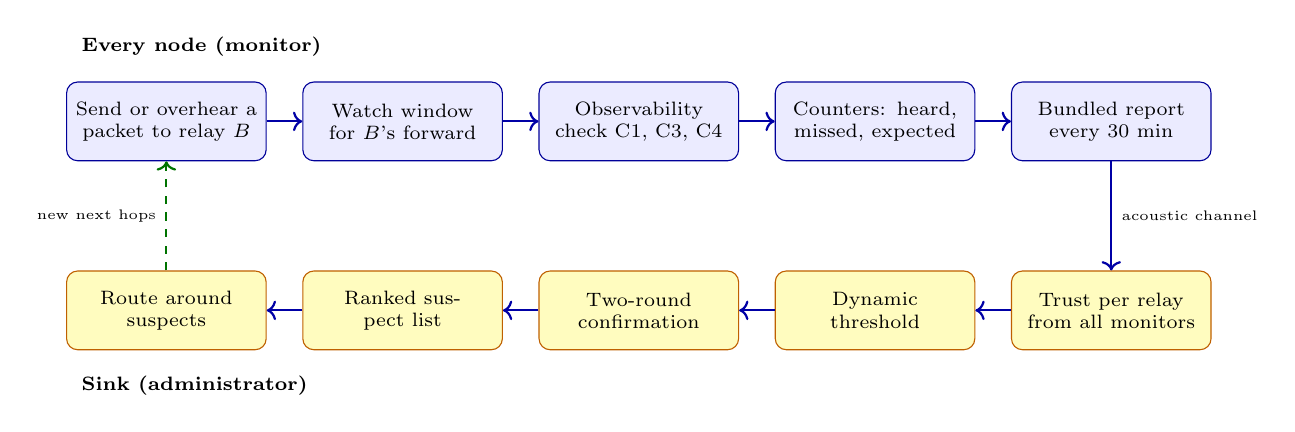
\begin{tikzpicture}[
  box/.style={draw=blue!60!black, fill=blue!8, rounded corners, align=center, font=\scriptsize, text width=2.3cm, minimum height=1.0cm},
  sink/.style={draw=orange!75!black, fill=yellow!25, rounded corners, align=center, font=\scriptsize, text width=2.3cm, minimum height=1.0cm},
  data/.style={->, thick, draw=blue!65!black},
  control/.style={->, thick, dashed, draw=green!45!black}]
\node[box] (obs) at (0,0) {Send or overhear a packet to relay $B$};
\node[box] (win) at (3.0,0) {Watch window for $B$'s forward};
\node[box] (chk) at (6.0,0) {Observability check C1, C3, C4};
\node[box] (cnt) at (9.0,0) {Counters: heard, missed, expected};
\node[box] (rep) at (12.0,0) {Bundled report every 30 min};
\node[sink] (tru) at (12.0,-2.4) {Trust per relay from all monitors};
\node[sink] (dec) at (9.0,-2.4) {Dynamic threshold};
\node[sink] (con) at (6.0,-2.4) {Two-round confirmation};
\node[sink] (lst) at (3.0,-2.4) {Ranked suspect list};
\node[sink] (rt) at (0,-2.4) {Route around suspects};
\node[font=\scriptsize\bfseries, anchor=west] at (-1.2,0.95) {Every node (monitor)};
\node[font=\scriptsize\bfseries, anchor=west] at (-1.2,-3.35) {Sink (administrator)};
\draw[data] (obs)--(win); \draw[data] (win)--(chk); \draw[data] (chk)--(cnt); \draw[data] (cnt)--(rep);
\draw[data] (rep)--node[right, font=\tiny]{acoustic channel}(tru);
\draw[data] (tru)--(dec); \draw[data] (dec)--(con); \draw[data] (con)--(lst); \draw[data] (lst)--(rt);
\draw[control] (rt.north)--node[left, font=\tiny]{new next hops}(obs.south);
\end{tikzpicture}}
\caption{Architecture of the proposed detector.}\label{fig:arch}
\end{figure}

\subsection{System and attack model}\label{sec:model}
\noindent
The network has 20 static sensors and one sink, placed at random in a 4~km by 4~km field and redrawn until every sensor reaches the sink within the 1500~m range. Each sensor sends to the nearest neighbour one hop closer to the sink. Node positions and the channel's distance loss are known. The busiest one, two or three relays are grayholes that drop each packet they should forward with probability $p = 0.3$ and still send their own data and reports. Monitors report truthfully and grayholes do not collude. Figure~\ref{fig:topology} shows one test network.

\begin{figure}[htbp]
\centering
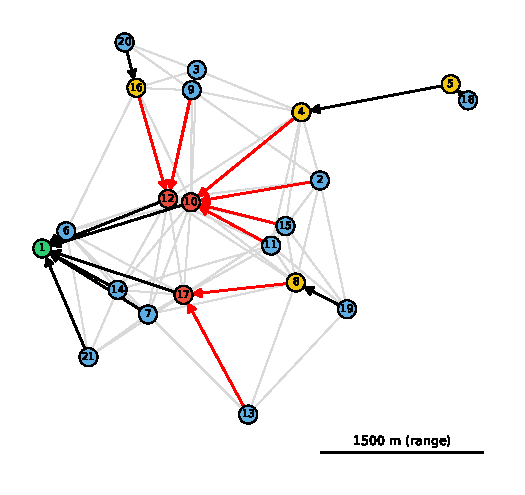
\includegraphics[width=0.34\linewidth]{figs/topology.pdf}
\caption{Test network 201. Node 1 (green) is the sink, blue nodes only send their own data, yellow nodes are honest relays and red nodes 10, 12 and 17 are grayholes. Arrows show each node's route; red arrows lead into a grayhole. Grey lines join nodes within range, which can overhear each other. Nodes 7 and 14 are 100~m apart and are drawn slightly apart.}\label{fig:topology}
\end{figure}

\subsection{Observability check}\label{sec:observability}
\noindent
Let $M$ be the monitor, $A$ the node that sent packet $P$ and $B$ the relay. A packet is identified by its origin and sequence number. When $M$ receives the end of $A$'s frame at time $t$, it computes from the known distances $d$ and the speed of sound $c$ when $P$ was arriving at $B$ and when $B$'s forward should reach $M$:
\begin{align}
t_A &= t - d(A,M)/c, \qquad (t_A = t \text{ when } M \text{ sent } P \text{ itself})\\
I_B &= \bigl[t_A + d(A,B)/c - T_f,\; t_A + d(A,B)/c\bigr],\\
W &= \bigl[\mathrm{end}(I_B) + d(B,M)/c,\; \mathrm{end}(I_B) + T_w + T_f + d(B,M)/c\bigr],
\end{align}
where $T_f \approx 1.02$~s is the frame duration and $T_w = 2$~s is the time a relay may hold a packet before forwarding it. In our networks 99\% of forwards left within 50~ms and the slowest took 1.12~s, so 2~s is a safe allowance. Figure~\ref{fig:window} shows the timing.

\begin{figure}[htbp]
\centering
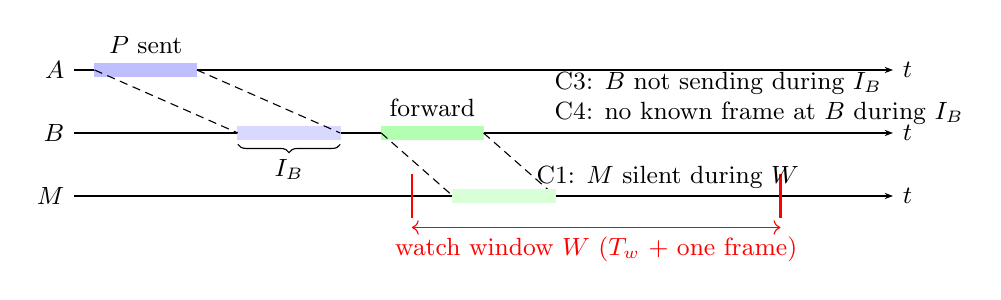
\begin{tikzpicture}[x=1.3cm, y=0.8cm, font=\small]
\foreach \y/\n in {2/A,1/B,0/M} {\draw[-{Stealth[length=3pt]}] (0,\y)--(8,\y) node[right]{$t$}; \node[left] at (0,\y) {$\n$};}
\fill[blue!25,draw] (0.2,1.9) rectangle (1.2,2.1); \node[above] at (0.7,2.1) {$P$ sent};
\fill[blue!15,draw] (1.6,0.9) rectangle (2.6,1.1);
\draw[densely dashed] (0.2,2)--(1.6,1); \draw[densely dashed] (1.2,2)--(2.6,1);
\draw[decorate,decoration={brace,amplitude=3pt,mirror}] (1.6,0.82)--(2.6,0.82) node[midway,below=2pt]{$I_B$};
\fill[green!30,draw] (3.0,0.9) rectangle (4.0,1.1); \node[above] at (3.5,1.1) {forward};
\draw[densely dashed] (3.0,1)--(3.7,0); \draw[densely dashed] (4.0,1)--(4.7,0);
\fill[green!15,draw] (3.7,-0.1) rectangle (4.7,0.1);
\draw[red,thick] (3.3,-0.35)--(3.3,0.35); \draw[red,thick] (6.9,-0.35)--(6.9,0.35);
\draw[red,<->] (3.3,-0.5)--node[below]{watch window $W$ ($T_w$ + one frame)}(6.9,-0.5);
\node[align=left,anchor=west] at (4.6,1.55) {C3: $B$ not sending during $I_B$\\C4: no known frame at $B$ during $I_B$};
\node at (5.8,0.3) {C1: $M$ silent during $W$};
\end{tikzpicture}
\caption{Watch window of monitor $M$ for relay $B$. Dashed lines show propagation at 1500~m/s.}\label{fig:window}
\end{figure}

\noindent
A window is kept only if three locally known conditions hold, decided without looking at whether the forward was heard. \textbf{C1:} $M$ did not transmit during $W$, since a half-duplex modem cannot receive while it sends. \textbf{C3:} $M$ did not hear $B$ transmit during $I_B$, since $B$ would then have been deaf to $P$. \textbf{C4:} no frame known to $M$, its own or one decoded from a neighbour other than $A$ and $B$, reached $B$ during $I_B$; a frame sent by $C$ during $[t_0,t_1]$ is at $B$ during $[t_0,t_1]+d(C,B)/c$. A kept window is HEARD if $M$ overheard $B$ forward $P$ inside $W$ and MISSED otherwise; an excluded window counts as neither. A corrupted frame at $M$ (C2) is deliberately not used, because the relay's own forward can cause it while a drop never does. On our calibration networks C2 held for 87.7\% of forwarding attempts but 98.4\% of drops.

\subsection{Expected forwards and trust}\label{sec:trust}
\noindent
Even a kept window can lose the forward to the channel. With the channel's frame loss at distance $d$ given by $e(d) = 0.15\,(d/1500)^2$, the chance that an honest forward reaches $M$ through the channel alone is
\begin{equation}
g_w = \bigl(1-e(d_{AB})\bigr)\bigl(1-e(d_{BM})\bigr).
\end{equation}
For each monitor and relay link $i$, let $n_i$ be the kept windows, $O_i$ the heard forwards and $G_i = \sum_w g_w$ the channel-only expectation. Collisions that the monitor cannot see still remove some forwards, so each link also has a residual loss
\begin{equation}
\kappa_i = \max\bigl(0,\, 1 - O_i/G_i\bigr).
\end{equation}
Links are grouped into near, medium and far areas by the tertiles of their length. For a relay $B$, the normal residual loss of an area is the median $\kappa$ of the other relays' links in that area, so $B$ cannot hide in its own baseline. The expected forwards on link $i$ and the trust and suspicion score of $B$ are then
\begin{equation}
E_i = G_i\bigl(1-\kappa_{\mathrm{area}(i),\,-B}\bigr), \qquad
T_B = \frac{\sum_i O_i}{\sum_i E_i}, \qquad
S_B = 100\,\max\bigl(0,\, 1 - T_B\bigr).
\end{equation}
$T_B$ is the weighted average of every monitor's own trust $O_i/E_i$, in which each monitor counts by the forwards it expected. If the expectation is right and the relay keeps each packet with probability $1-p$, then the expected value of $O$ is $(1-p)E$, so $S_B$ estimates the drop rate in percent.

\subsection{Dynamic threshold and confirmation}\label{sec:decision}
\noindent
The shortfall of relay $B$ in standard deviations is
\begin{equation}
z_B = \frac{\sum_i E_i - \sum_i O_i}{\sqrt{\sum_i E_i \max\bigl(0.01,\, 1-E_i/n_i\bigr)}}.
\end{equation}
Monitors watching the same packet are correlated, so each $z_B$ is divided by $\sqrt{\phi}$, where $\phi = \max(1, m/0.455)$ and $m$ is the median of $z_B^2$ over relays with $z_B<0$. For $k$ judged relays the threshold is $z^* = \Phi^{-1}(1-\alpha/k)$. A relay is flagged when it has at least 20 kept windows, $S_B \geq 10$ and $z_B > z^*$. We chose $\alpha = 10^{-4}$ on tuning networks never used for testing; because of the correlation it is a tuning knob, not a proven false-alarm probability.

Several grayholes in one area raise its normal loss, inflate $\phi$ and hide one another. The detector therefore removes relays with $S_B \geq 10$ and confirmed suspects from the area medians and repeats the estimate, at most three times. A relay becomes a suspect only when flagged in two consecutive 30-minute rounds, and stays one until the administrator reviews it.

\subsection{Algorithm}\label{sec:algo}
\noindent
Every node runs the observability check of Section~\ref{sec:observability} on each window and sends its counters at each checkpoint; Section~\ref{sec:impl} gives that code. Algorithm~\ref{alg:sink} is the decision the sink makes every 30 minutes.

\begin{algorithm}[htbp]
\small
\caption{Decision at the sink (every 30 min)}\label{alg:sink}
\begin{algorithmic}[1]
\State $R \gets$ latest delivered report of every monitor and relay link, plus the sink's own counters
\State $X \gets$ confirmed suspects
\Repeat \Comment{baseline cleaning, at most 3 times}
  \For{each link $i$ with $n_i \geq 5$} \State $\kappa_i \gets \max(0, 1-O_i/G_i)$ \EndFor
  \For{each relay $B$}
    \State $E_i \gets G_i(1 - \mathrm{median}\{\kappa_j : j \text{ in same area}, \text{relay}(j) \notin X \cup \{B\}\})$
    \State $T_B \gets \sum O_i / \sum E_i$; \; $S_B \gets 100\max(0, 1-T_B)$; \; compute $z_B$
  \EndFor
  \State Rescale $z$ by $\sqrt{\phi}$; \; $X \gets$ confirmed suspects $\cup \{B : S_B \geq 10\}$
\Until{$X$ does not change}
\State $F \gets \{B : n_B \geq 20,\ S_B \geq 10,\ z_B > z^*\}$
\State $\mathit{suspects} \gets \mathit{suspects} \cup (F \cap F_{\mathrm{previous}})$; \; $F_{\mathrm{previous}} \gets F$
\State Give the administrator the relays ranked by $S_B$; route around $\mathit{suspects}$ where another path exists
\end{algorithmic}
\end{algorithm}


\subsection{Justification of design choices}\label{sec:justify}
\begin{itemize}
  \item \textbf{Observability before outcome.} C1, C3 and C4 use only timing the monitor records and apply to heard and missed forwards alike, so the filter favours neither. Every neighbour watches, so relays are judged on more windows at no cost.
  \item \textbf{Expected forwards per link, area median from other relays.} Far links lose more frames than near ones even when every relay is honest. The median ignores a minority of bad links, and leaving out the judged relay stops a grayhole from raising its own baseline; a weighted average lowered single-grayhole recall from 96\% to 75\% in a single-round tuning test.
  \item \textbf{Dynamic threshold and baseline cleaning.} The threshold follows the number of judged relays and the spread of the round. Cleaning raised three-grayhole detection on the calibration networks from 4 of 18 to 13 of 18.
  \item \textbf{Two-round confirmation and avoidance.} One noisy round accuses nobody, and routing around suspects instead of cutting them off keeps nodes connected when a grayhole is their only path.
\end{itemize}

%==========================================================
\section{Implementation}\label{sec:impl}

\subsection{Tools and environment}
\noindent
The detector is implemented in UnetStack 7.0.0, community edition, on Java 8, with agents and scripts in Groovy \cite{chitre2014}. Each node's agent subscribes to UnetStack's physical-layer notifications: \texttt{TxFrameNtf} when its own frame leaves and \texttt{RxFrameNtf} when it decodes a frame, including frames for other nodes \cite{unethandbook}. Python with matplotlib draws the graphs. \texttt{run.sh} runs four steps: \texttt{record.groovy} records every monitor's counters, \texttt{compare.groovy} replays the sink's decisions for every method on the same counters, \texttt{network.groovy} runs the live network and \texttt{analysis/plots.py} draws the graphs.

\subsection{Class diagram}
\noindent
Figure~\ref{fig:classes} shows the classes and how the simulation scripts use them. \texttt{MonitorNode} extends UnetStack's \texttt{UnetAgent}, and \texttt{DistanceLossChannel} extends its \texttt{ProtocolChannelModel}. \texttt{Detectors} holds all three detection methods as static functions, so every method reads exactly the same evidence.

\begin{figure}[htbp]
\centering
\resizebox{\linewidth}{!}{%
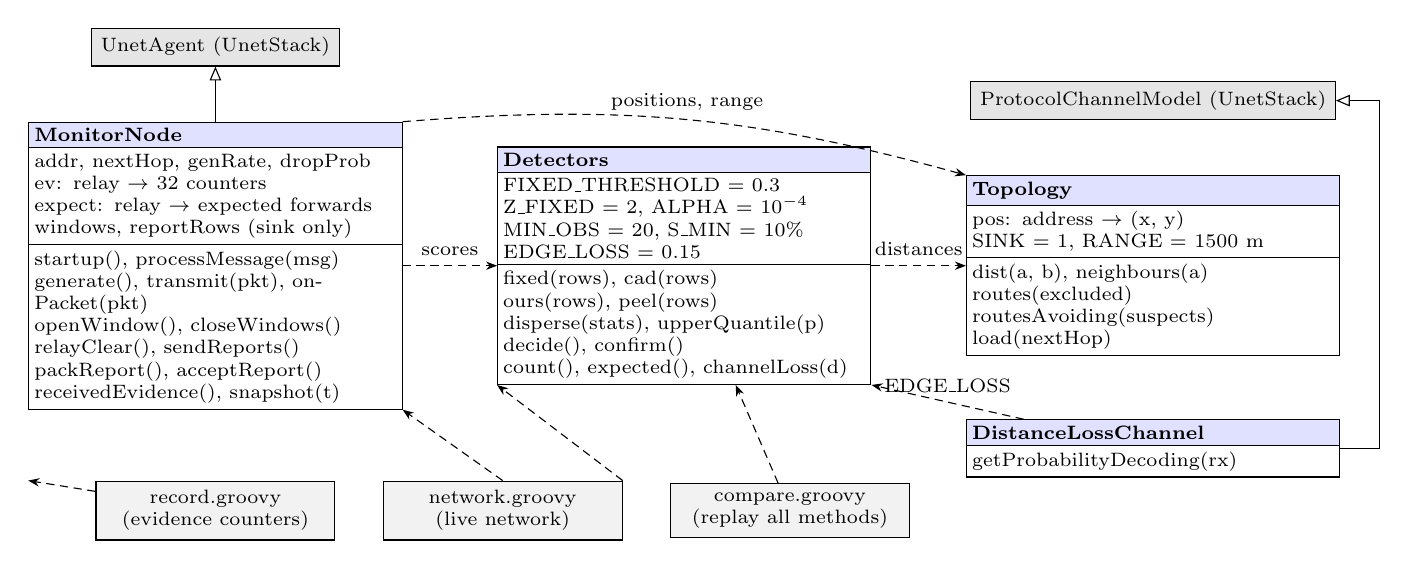
\begin{tikzpicture}[font=\scriptsize,
  cls/.style={draw, rectangle split, rectangle split parts=3, rectangle split part fill={blue!12,white,white}, align=left, text width=4.6cm, inner sep=2pt},
  scr/.style={draw, fill=gray!10, align=center, text width=2.8cm, minimum height=0.6cm},
  uses/.style={-{Stealth[length=4pt]}, densely dashed},
  inh/.style={-{Triangle[open,length=5pt]}}]
\node[cls] (mon) at (0,0) {\centering\textbf{MonitorNode}
\nodepart{second}addr, nextHop, genRate, dropProb\\ev: relay $\to$ 32 counters\\expect: relay $\to$ expected forwards\\windows, reportRows (sink only)
\nodepart{third}startup(), processMessage(msg)\\generate(), transmit(pkt), onPacket(pkt)\\openWindow(), closeWindows()\\relayClear(), sendReports()\\packReport(), acceptReport()\\receivedEvidence(), snapshot(t)};
\node[cls, right=1.2cm of mon] (det) {\centering\textbf{Detectors}
\nodepart{second}FIXED\_THRESHOLD = 0.3\\Z\_FIXED = 2, ALPHA = $10^{-4}$\\MIN\_OBS = 20, S\_MIN = 10\%\\EDGE\_LOSS = 0.15
\nodepart{third}fixed(rows), cad(rows)\\ours(rows), peel(rows)\\disperse(stats), upperQuantile(p)\\decide(), confirm()\\count(), expected(), channelLoss(d)};
\node[cls, right=1.2cm of det] (top) {\centering\textbf{Topology}
\nodepart{second}pos: address $\to$ (x, y)\\SINK = 1, RANGE = 1500 m
\nodepart{third}dist(a, b), neighbours(a)\\routes(excluded)\\routesAvoiding(suspects)\\load(nextHop)};
\node[draw, fill=gray!20, above=0.7cm of mon] (ua) {UnetAgent (UnetStack)};
\node[cls, rectangle split parts=2, below=0.8cm of top] (ch) {\centering\textbf{DistanceLossChannel}
\nodepart{second}getProbabilityDecoding(rx)};
\node[draw, fill=gray!20, above=0.7cm of top] (pcm) {ProtocolChannelModel (UnetStack)};
\node[scr, below=0.9cm of mon] (rec) {record.groovy\\(evidence counters)};
\node[scr, right=0.6cm of rec] (net) {network.groovy\\(live network)};
\node[scr, right=0.6cm of net] (cmp) {compare.groovy\\(replay all methods)};
\draw[inh] (mon)--(ua);
\draw[inh] (ch.east)--++(0.5,0)|-(pcm.east);
\draw[uses] (mon)--node[above]{scores}(det);
\draw[uses] (det)--node[above]{distances}(top);
\draw[uses] (mon.north east) to[bend left=10] node[above]{positions, range} (top.north west);
\draw[uses] (rec)--(mon.south west|-rec.north);
\draw[uses] (net.north)--(mon.south east);
\draw[uses] (net.north east)--(det.south west);
\draw[uses] (cmp)--(det);
\draw[uses] (ch)--node[above]{EDGE\_LOSS}(det.south east);
\end{tikzpicture}}
\caption{Class diagram. Open arrow heads show inheritance and dashed arrows show use.}\label{fig:classes}
\end{figure}

\subsection{Node agent and the attack}
\noindent
\texttt{startup()} plays the role of a \texttt{main()} function. It finds the physical-layer agent, subscribes to its notifications and adds three behaviours: a Poisson generator for the node's own data, a 200~ms ticker that closes finished windows and a 30-minute ticker for the checkpoint. A data packet is 8 bytes: origin, sequence number, generation time and hop count. \texttt{onPacket()} carries out the attack, as Algorithm~\ref{alg:onpacket} shows. The sink records deliveries and stores reports; every other node forwards the packet unless it is a grayhole and the random draw says drop.

\begin{algorithm}[htbp]
\small
\caption{\texttt{startup()} and \texttt{onPacket()} in \texttt{MonitorNode}}\label{alg:onpacket}
\begin{algorithmic}[1]
\Function{startup}{}
  \State $\mathit{phy} \gets$ agent for the PHYSICAL service; subscribe to its topic and to DATAGRAM
  \State Add PoissonBehavior($1/\mathit{genRate}$) calling \textsc{generate}
  \State Add TickerBehavior(200 ms) calling \textsc{closeWindows}
  \State Add TickerBehavior(30 min) calling \textsc{snapshot}, \textsc{sendReports} and, at the sink, \textsc{onRound}
\EndFunction
\Function{onPacket}{$\mathit{pkt}$}
  \If{this node is the sink}
    \If{$\mathit{pkt}$ is a report} \State \textsc{acceptReport}($\mathit{pkt}$) \Else \State record delivery and latency \EndIf
    \State \Return
  \EndIf
  \If{$\mathit{dropProb} > 0$ \textbf{and} random() $< \mathit{dropProb}$} \State \Return \Comment{grayhole drops it} \EndIf
  \State $\mathit{pkt}.\mathit{hops} \gets \mathit{pkt}.\mathit{hops}+1$; \textsc{transmit}($\mathit{pkt}$) to $\mathit{nextHop}$
\EndFunction
\end{algorithmic}
\end{algorithm}

\subsection{Watch windows and the observability check}
\noindent
\texttt{processMessage()} handles the notifications. When the node's own frame leaves, it records the transmission interval and opens a window for its next hop. When it decodes a frame for another node, it records the sender's transmission interval, marks a matching open window as heard and opens a window for the frame's destination. \texttt{closeWindows()} and \texttt{relayClear()} implement C1, C3 and C4 (Algorithm~\ref{alg:close}). Each outcome goes into one of 32 counter bins that record whether the monitor was the sender, which conditions failed and whether the forward was heard. Keeping all 32 bins lets the same recorded evidence feed the fixed watchdog (sender windows only), the CAD-style detector and our detector with and without the filter.

\begin{algorithm}[htbp]
\small
\caption{\texttt{closeWindows()} and \texttt{relayClear()} in \texttt{MonitorNode}}\label{alg:close}
\begin{algorithmic}[1]
\Function{closeWindows}{}
  \For{each window $w$ with now $> \mathrm{end}(W) + 50$ ms}
    \State $c_{13} \gets$ not overlaps($\mathit{myTx}$, $W$) \textbf{and} not overlaps($\mathit{heardTx}[B]$, $I_B$)
    \State $c_2 \gets$ not overlaps($\mathit{badFrames}$, $W$) \Comment{stored, not used by our detector}
    \State $c_4 \gets$ \textsc{relayClear}($w$)
    \State $i \gets$ idx($\mathit{sender}, c_{13}, c_2, c_4, \mathit{heard}$); \; $\mathit{ev}[B][i] \gets \mathit{ev}[B][i] + 1$
    \State $\mathit{expect}[B][i] \gets \mathit{expect}[B][i] + (1-e(d(A,B)))(1-e(d(B,M)))$
    \State Remove $w$
  \EndFor
\EndFunction
\Function{relayClear}{$w$}
  \For{each node $C$ with known frames ($M$'s own and decoded neighbours), $C \notin \{A, B\}$, $d(C,B) \leq$ range}
    \State $s \gets d(C,B)/c$
    \If{any frame $[t_0,t_1]$ of $C$ has $[t_0+s, t_1+s]$ overlapping $I_B$} \State \Return false \EndIf
  \EndFor
  \State \Return true
\EndFunction
\end{algorithmic}
\end{algorithm}

\subsection{Reports and the decision at the sink}
\noindent
At each checkpoint a node freezes its counters and bundles them into one report frame. The frame has a 12-byte header (the 8-byte packet header plus a 32-bit busy fraction) and one 17-byte entry per watched relay: relay identifier, two 32-bit counts and a 64-bit expected-forward sum. Up to six entries, 114 bytes, fit into the simulator's 128-byte data frame. Reports are spread over ten minutes after the checkpoint to reduce collisions between them, and they travel to the sink like data, so they can be lost or dropped by a grayhole. \texttt{acceptReport()} rejects malformed entries, duplicates and reports older than the one already held. The sink keeps the latest delivered report of every link. Counters are cumulative, so a lost report only delays evidence.

\texttt{Detectors.ours()} implements Section~\ref{sec:trust} and Section~\ref{sec:decision}, \texttt{peel()} repeats it for baseline cleaning and \texttt{confirm()} applies the two-round rule. After each round the sink calls \texttt{routesAvoiding()}, which gives each node the shortest route that avoids the suspects. A node with no such route keeps its old one.

\subsection{Baselines, channel and pipeline}
\noindent
Both baselines use the same agent, reports, confirmation and rerouting, so only the detection rule differs. The fixed watchdog uses sender windows and accuses a relay whose miss rate exceeds 30\%. The CAD-style detector uses sender windows with normal loss $p_r = 1-(1-e(d))^2(1-p_o)^2$, where $p_o = 1-(1-R_b)^2$ comes from the monitor's busy ratio $R_b$, and flags a relay when a pooled binomial $z$ exceeds 2. \texttt{DistanceLossChannel} overrides one method of the protocol channel model so that a frame at distance $d$ decodes with probability $1-0.15\,(d/1500)^2$. \texttt{./run.sh demo} runs one live network with three grayholes in about three minutes and prints the ranked suspect list; \texttt{./run.sh} regenerates every number and graph in about an hour.

%==========================================================
\section{Results and analysis}\label{sec:results}

\subsection{Simulation parameters}
\begin{table}[htbp]
\centering\small\setstretch{1.0}
\caption{Simulation parameters.}\label{tab:params}
\begin{tabular}{>{\raggedright\arraybackslash}p{3.4cm} >{\raggedright\arraybackslash}p{10.3cm}}
\toprule
Parameter & Value \\
\midrule
Simulator & UnetStack 7.0.0 community edition, Java 8 \\
Channel & Protocol channel model, range 1500 m, decoding probability $1-0.15(d/1500)^2$ \\
Sound speed, frame & 1500 m/s; 128-byte data frame of about 1.02 s \\
Network, routing & 20 sensors and one sink in 4 km $\times$ 4 km at 50 m depth; shortest hop count \\
Traffic, grayholes & Poisson, 0.001 to 0.01 packets/s per sensor (0.005 default); 1 to 3 busiest relays drop 30\% \\
Timing & $T_w = 2$ s; decision every 30 min; 6 h recorded and 12 h live runs \\
Networks & Tuning topologies 101--106; test topologies 201--210 \\
Own thresholds & Fixed watchdog miss rate $> 0.3$; CAD-style $z > 2$; ours $\alpha = 10^{-4}$ \\
Same-budget thresholds & Fixed 0.6; CAD-style $z > 2.5$; ours $\alpha = 10^{-4}$ \\
Response & Suspects stop relaying wherever another path exists \\
\bottomrule
\end{tabular}
\end{table}

\subsection{Scenarios}
\noindent
The recorded runs cover eight scenarios on every test topology. \emph{Load} has one 30\% grayhole at four traffic loads, each with a no-attack twin. \emph{Drop} has one grayhole dropping 10, 20, 50 or 100\%. \emph{Two} and \emph{three} make the two or three busiest relays grayholes. \emph{Near} attacks the relay with the closest neighbours. In \emph{hotspot}, three well-connected sensors send six times as much as the others at the same total traffic. \emph{Large} has 40 sensors in 6~km by 6~km and \emph{sparse} 20 sensors in 5~km by 5~km. The 12-hour live network adds reports, detection and rerouting for one grayhole at loads 0.005 and 0.01 and for two and three grayholes.
\subsection{Performance metrics}
\noindent
We measure the share of grayholes confirmed as suspects by the end of a run, the honest relays confirmed as suspects, the delivery ratio of honest data packets (the grayholes' own packets excluded), the throughput in honest packets delivered per hour with all report traffic on the channel, the time until every grayhole is confirmed, and the report frames sent. A topology is the independent unit. Intervals are 95\% $t$-intervals over the ten test topologies, paired by topology when two methods are compared.

\subsection{Effect of the attack}
\noindent
Figure~\ref{fig:bars}(a) shows how much honest delivery the attack costs with no defence, compared with the same network without attack. One grayhole costs 8.4 percentage points, two cost 14.2 and three cost 17.0. Each added grayhole costs less than the one before, since the busiest relay is attacked first and the later ones carry less traffic.

\begin{figure}[htbp]
\centering
\begin{minipage}{0.3\linewidth}\centering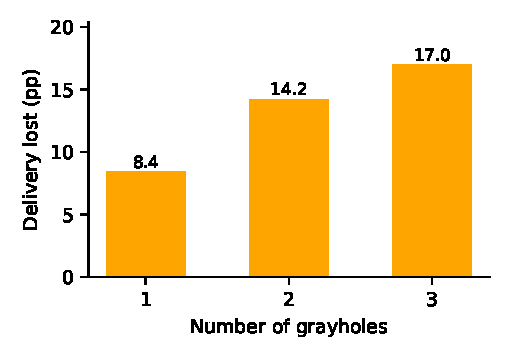
\includegraphics[width=\linewidth]{figs/attack.pdf}\\(a)\end{minipage}\qquad
\begin{minipage}{0.3\linewidth}\centering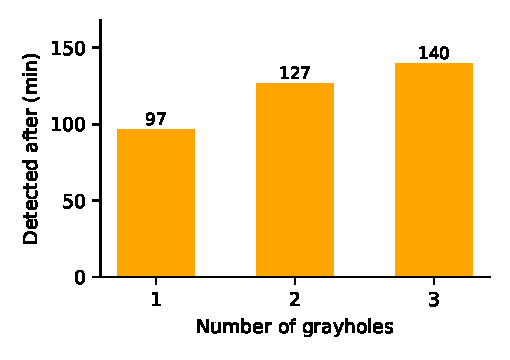
\includegraphics[width=\linewidth]{figs/detect_time.pdf}\\(b)\end{minipage}
\caption{For 1, 2 and 3 grayholes: (a) honest delivery lost to the attack in percentage points (live network, no defence); (b) time until our detector confirmed every grayhole, over the runs in which this happened.}\label{fig:bars}
\end{figure}

\subsection{Detection of grayholes}
\noindent
Our detector confirmed 90\% of single grayholes, 95\% of grayholes in networks with two and 77\% in networks with three. Confirmation needs two flagged rounds, so the earliest possible time is 60 minutes; Figure~\ref{fig:bars}(b) shows the mean rising from 97 to 140 minutes as grayholes are added, because several grayholes hide one another until the baseline has been cleaned.

Figure~\ref{fig:fig3}(a) is the fair contest. Every method's threshold was tuned on the tuning networks so that at most 5\% of honest relays are accused without an attacker, then applied unchanged to the test networks. At the same budget, our detector found 90\% of single grayholes against 58\% for the CAD-style detector and 22\% for the fixed watchdog. With two grayholes it found 95\% against 65\% and 40\%. With three grayholes it tied the CAD-style detector at 77\%. Figure~\ref{fig:fig3}(b) shows each method with its own rule: the fixed watchdog reaches 100\% detection only by accusing 41 to 71\% of honest relays.

\begin{figure}[htbp]
\centering
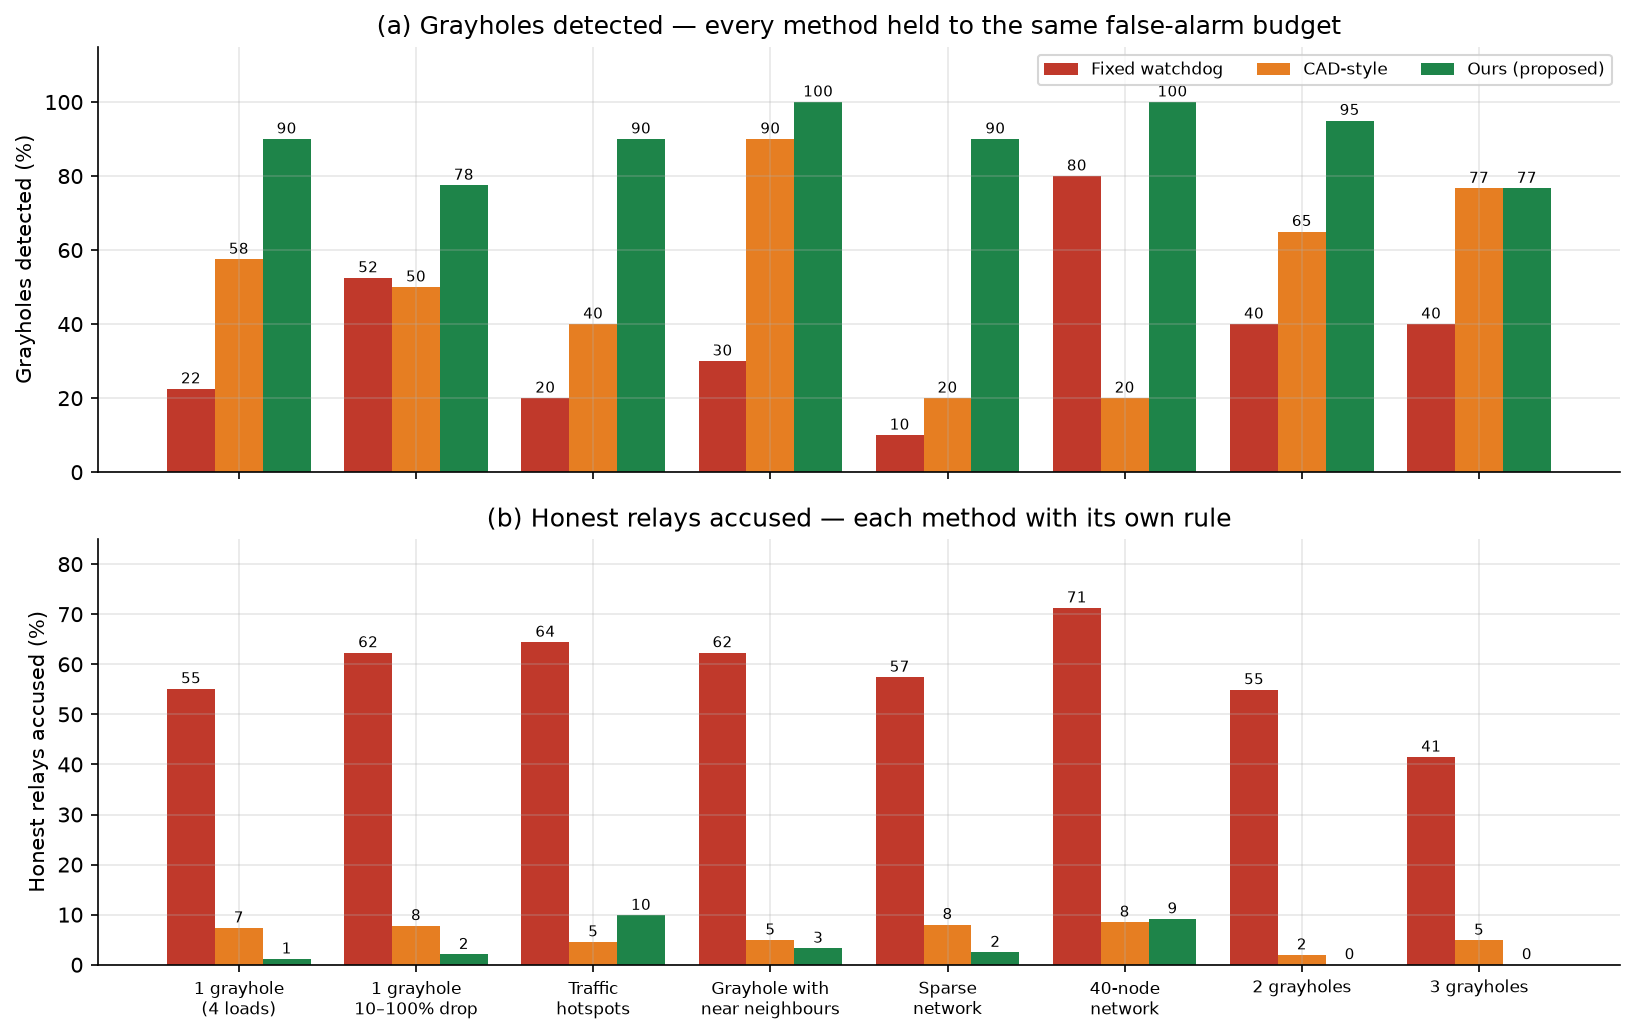
\includegraphics[width=0.45\linewidth]{figs/fig3_detection.png}
\caption{(a) Grayholes detected with every method held to the same false-alarm budget; (b) honest relays accused with each method's own rule (6 h, ten test topologies).}\label{fig:fig3}
\end{figure}

\subsection{False accusations}
\noindent
Figure~\ref{fig:fig2} explains why the fixed watchdog fails. With no attacker at all, it accused 1.0 honest relay per run at the lowest load and 6.2 at the highest, because collisions and half-duplex deafness grow with traffic and it counts them as drops. The CAD-style detector accused 0.3 to 0.7, and our detector 0 to 0.1.

\begin{figure}[htbp]
\centering
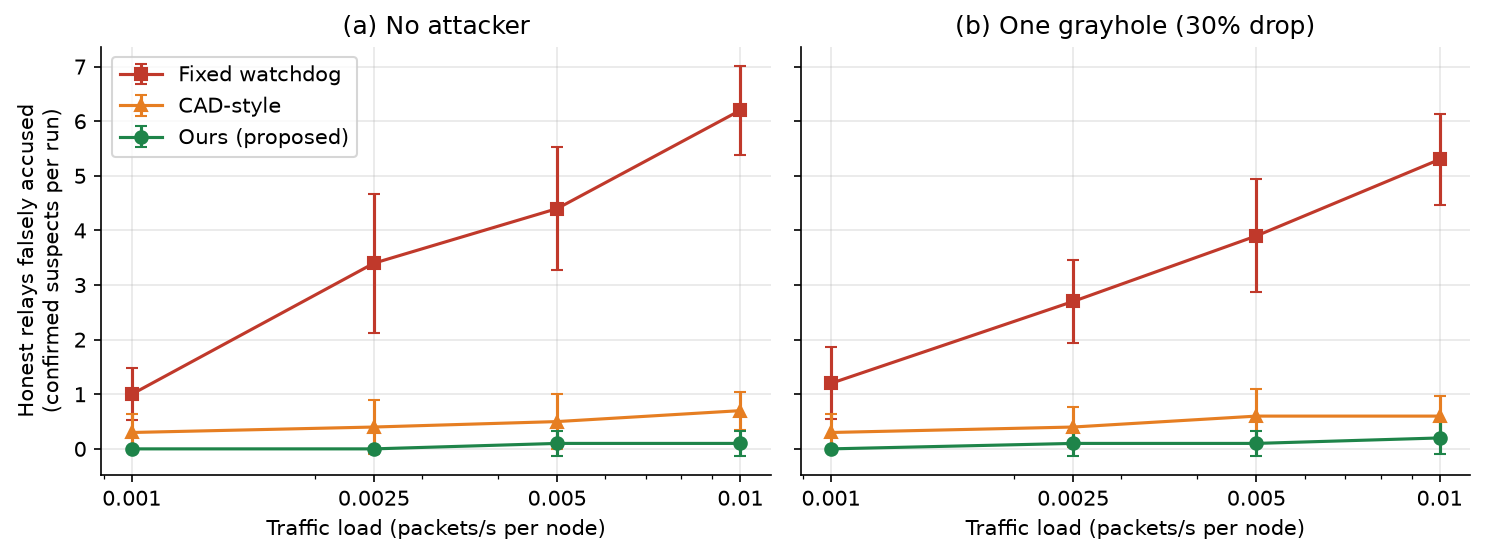
\includegraphics[width=0.5\linewidth]{figs/fig2_false_accusations.png}
\caption{Honest relays falsely accused per run against traffic load, each method with its own rule (6 h, ten test topologies, 95\% intervals).}\label{fig:fig2}
\end{figure}

\subsection{Ranked suspect list and drop estimate}
\noindent
Figure~\ref{fig:fig4}(a) is the list the administrator receives for the network of Figure~\ref{fig:topology} after six hours. The three grayholes rank first with estimated drop rates of 38.9, 32.1 and 28.2\% and are confirmed. Every honest relay is estimated at 0 to 0.2\%. Figure~\ref{fig:fig4}(b) shows that the estimate follows the true drop rate: 7.6, 18.8 and 47.2\% for true rates of 10, 20 and 50\%. The CAD-style score gives 0.0, 1.2 and 31.3\% for the same cases, so it underestimates moderate dropping.

\begin{figure}[htbp]
\centering
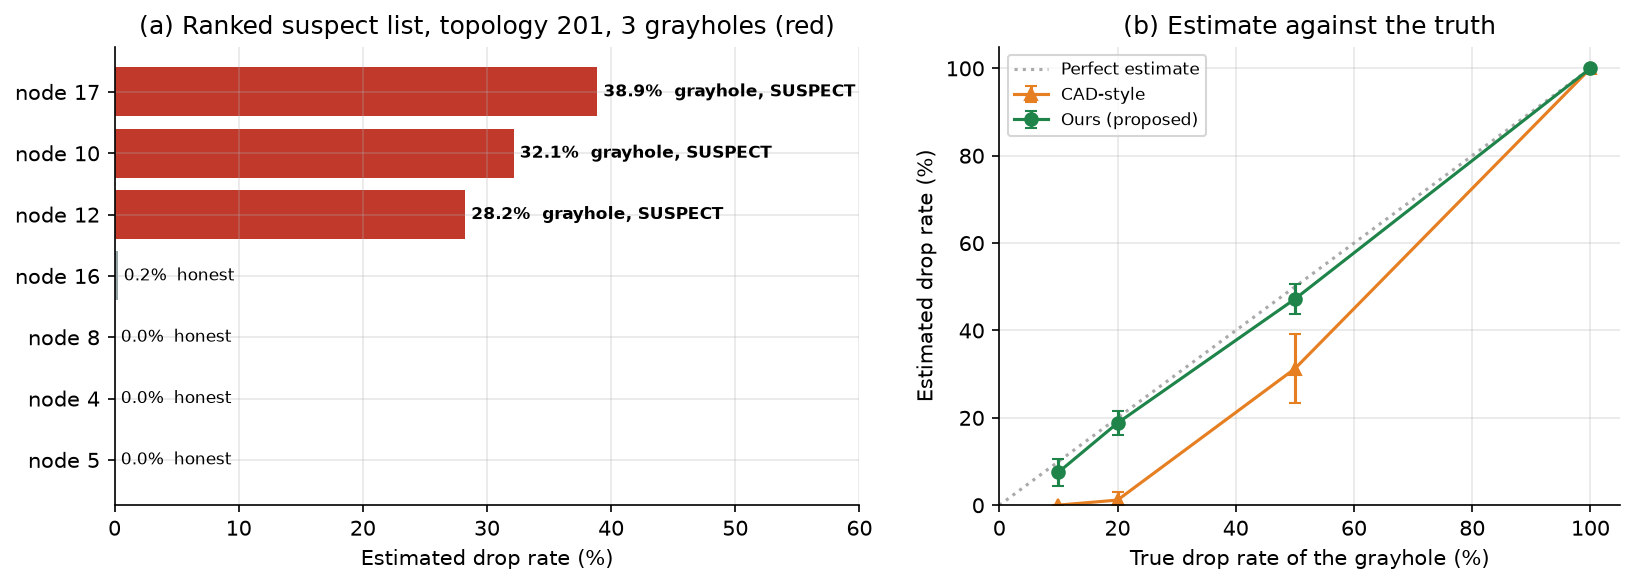
\includegraphics[width=0.6\linewidth]{figs/fig4_suspect_list.png}
\caption{(a) Ranked suspect list for test topology 201 with three grayholes; (b) estimated against true drop rate of one grayhole (load 0.005, ten test topologies).}\label{fig:fig4}
\end{figure}

\subsection{Network performance}
\noindent
Table~\ref{tab:live} pools every live-network setting. The fixed watchdog catches every grayhole, but it also routes around 7.2 honest relays per run, and the detours eat most of the gain: delivery rises only from 45.6 to 47.0\%. The CAD-style detector accuses fewer honest relays but misses 42\% of the grayholes. Our detector catches 95\% of the grayholes, accuses 0.3 honest relays per run and gives the highest delivery ratio and throughput. It sends about 10\% more report frames than the baselines (857 to 973 against 781 to 886 per run), because every monitor reports on every relay it overhears.

\begin{table}[htbp]
\centering\small\setstretch{1.0}
\caption{Live network, 12 h, ten test topologies, all settings pooled.}\label{tab:live}
\begin{tabular}{l c c c c}
\toprule
Method & Caught (\%) & Honest accused per run & Delivery (\%) & Throughput (pkt/h) \\
\midrule
No attack & n/a & n/a & 57.0 & 228.6 \\
Attack, no defence & 0 & 0 & 45.6 & 186.8 \\
Fixed watchdog & 100 & 7.2 & 47.0 & 190.6 \\
CAD-style & 58.3 & 0.8 & 48.0 & 193.3 \\
\textbf{Ours} & \textbf{95.0} & \textbf{0.3} & \textbf{49.7} & \textbf{200.5} \\
\bottomrule
\end{tabular}
\end{table}

\noindent
Figure~\ref{fig:fig5}(a) breaks delivery down by setting. Our detector is highest in all four, gaining 4.0, 1.7, 5.6 and 4.9 percentage points over no defence (interval above zero in three of four) and 4.0 points over the fixed watchdog with two and three grayholes. Its lead over the CAD-style detector, 0.7 to 2.7 points, is within the uncertainty. Figure~\ref{fig:fig5}(b) shows the mechanism over time with three grayholes: delivery falls when the attack starts and recovers once the grayholes are confirmed. In Figure~\ref{fig:fig5}(c) suspects are cut off instead of avoided. Every honest relay the fixed watchdog accuses is then lost together with the nodes behind it, and its delivery falls to 23.2\%, half the 45.6\% of no defence.

\begin{figure}[htbp]
\centering
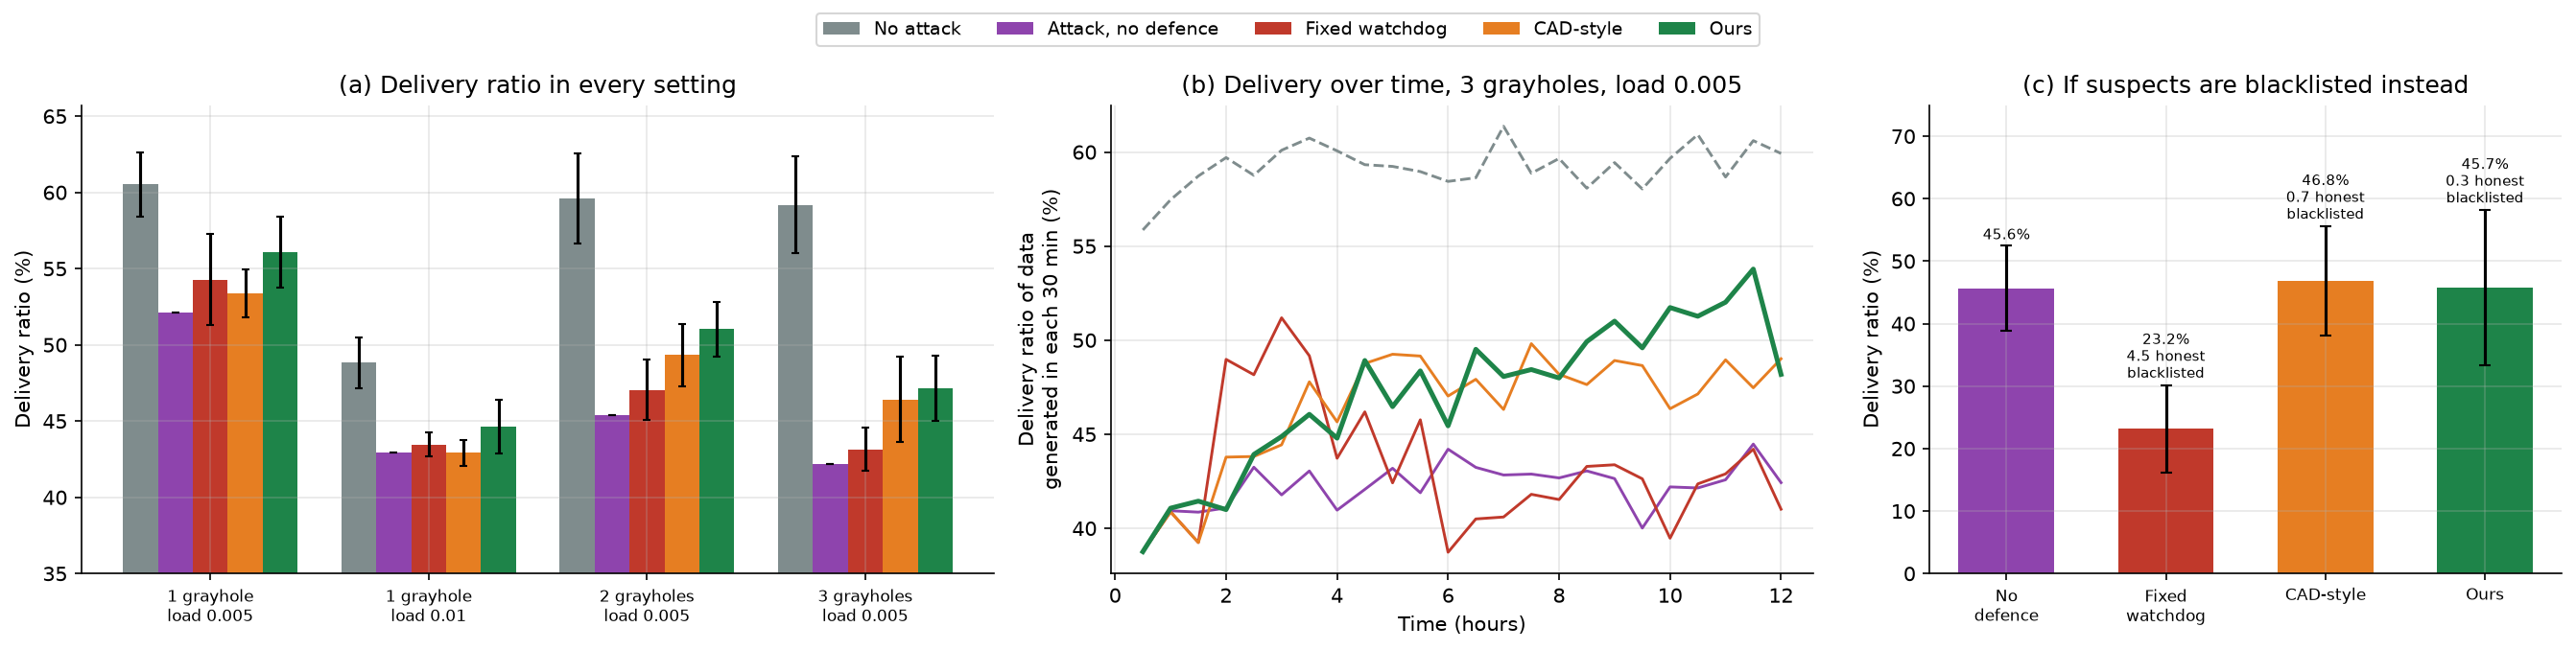
\includegraphics[width=0.72\linewidth]{figs/fig5_network_performance.png}
\caption{Live network: (a) delivery ratio per setting, with paired 95\% intervals against no defence; (b) delivery over time with three grayholes; (c) delivery when suspects are cut off instead of avoided.}\label{fig:fig5}
\end{figure}

\subsection{Comparison with existing approaches}
\noindent
The fixed watchdog and the CAD-style detector were measured above; both are adaptations, without the pathrater and with only CAD's downstream estimate. The other reviewed approaches were not implemented, so we compare them by what they report and need. The UnetStack3 detector \cite{brc2021} only says whether an attack happened and uses one monitor on four nodes. ARTMM \cite{han2015}, TAFLRLR \cite{han2023} and ATEM \cite{liu2024} name low-trust nodes but exchange recommendations and judge every failed interaction, or skip whole cycles, rather than each unobservable window. Our detector names the suspects with a drop estimate, needs one bundled report per node every 30 minutes and caught 95\% of the grayholes while accusing 0.3 honest relays per run.

\subsection{Contribution of each part and limits}
\noindent
Removing one part at a time at the same 5\% budget, three-grayhole detection falls from 23 of 30 to 17 of 30 without baseline cleaning. Without the observability filter detection barely changes once two-round confirmation is in place, but honest accusations rise from 1.1 to 1.5\% in the load sweep; the filter's main effect is the low count in Figure~\ref{fig:fig2}. Its limits are static topologies, a known loss curve, truthful monitors and free route updates; in hotspot and 40-node networks it accuses about 10\% of honest relays at the same budget, and with three grayholes it only ties the CAD-style detector.

%==========================================================
\section{Conclusions and future work}\label{sec:conclusion}
\noindent
The purpose of this work was to detect grayhole relays in underwater acoustic networks without accusing honest relays whose forwards were lost to half-duplex deafness, collisions or long links. We built in UnetStack a detector that counts a watch window only when the monitor could observe the forward, compares the forwards heard with the number each link should show, and flags relays with a dynamic threshold and two-round confirmation. Reports reach the sink over the acoustic channel, and the sink ranks the suspects and routes around them.

On ten test networks the detector caught 95\% of the grayholes while accusing 0.3 honest relays per run, against 7.2 for the fixed watchdog. At the same false-alarm budget it detected 90\% of single grayholes, against 58\% for the CAD-style detector and 22\% for the fixed watchdog. Its drop estimate tracked the true rate within three points, and it gave the highest delivery ratio, 49.7\% against 45.6\% with no defence.

Future work should test monitors that send false reports, mobile nodes and position errors, learn the loss curve online, reduce false accusations in dense networks and implement the published comparators in full.

%==========================================================
\begin{thebibliography}{99}

\bibitem{akyildiz2005}
I. F. Akyildiz, D. Pompili, and T. Melodia,
``Underwater acoustic sensor networks: research challenges,''
\emph{Ad Hoc Networks}, vol. 3, no. 3, pp. 257--279, 2005,
doi: 10.1016/j.adhoc.2005.01.004.

\bibitem{karlof2003}
C. Karlof and D. Wagner,
``Secure routing in wireless sensor networks: attacks and countermeasures,''
\emph{Ad Hoc Networks}, vol. 1, no. 2--3, pp. 293--315, 2003,
doi: 10.1016/S1570-8705(03)00008-8.

\bibitem{domingo2011}
M. C. Domingo,
``Securing underwater wireless communication networks,''
\emph{IEEE Wireless Communications}, vol. 18, no. 1, pp. 22--28, 2011,
doi: 10.1109/MWC.2011.5714022.

\bibitem{jiang2019}
S. Jiang,
``On securing underwater acoustic networks: a survey,''
\emph{IEEE Communications Surveys \& Tutorials}, vol. 21, no. 1, pp. 729--752, 2019,
doi: 10.1109/COMST.2018.2864127.

\bibitem{marti2000}
S. Marti, T. J. Giuli, K. Lai, and M. Baker,
``Mitigating routing misbehavior in mobile ad hoc networks,''
in \emph{Proc. 6th ACM MobiCom}, 2000, pp. 255--265,
doi: 10.1145/345910.345955.

\bibitem{shila2010}
D. M. Shila, Y. Cheng, and T. Anjali,
``Mitigating selective forwarding attacks with a channel-aware approach in WMNs,''
\emph{IEEE Transactions on Wireless Communications}, vol. 9, no. 5, pp. 1661--1675, 2010,
doi: 10.1109/TWC.2010.05.090700.

\bibitem{han2015}
G. Han, J. Jiang, L. Shu, and M. Guizani,
``An attack-resistant trust model based on multidimensional trust metrics in underwater acoustic sensor network,''
\emph{IEEE Transactions on Mobile Computing}, vol. 14, no. 12, pp. 2447--2459, 2015,
doi: 10.1109/TMC.2015.2402120.

\bibitem{brc2021}
B. R. Chandavarkar and N. Suresh,
``Demonstration of selective forwarding attack and detection mechanism in UnetStack3,''
in \emph{Proc. 12th Int. Conf. Computing Communication and Networking Technologies (ICCCNT)}, 2021, pp. 1--6,
doi: 10.1109/ICCCNT51525.2021.9580125.

\bibitem{han2023}
D. Han, X. Du, L. Wang, X. Liu, and X. Tian,
``Trust-aware and fuzzy logic-based reliable layering routing protocol for underwater acoustic networks,''
\emph{Sensors}, vol. 23, no. 23, art. 9323, 2023,
doi: 10.3390/s23239323.

\bibitem{liu2024}
C. Liu, J. Ye, F. An, and W. Jiang,
``An adaptive trust evaluation model for detecting abnormal nodes in underwater acoustic sensor networks,''
\emph{Sensors}, vol. 24, no. 9, art. 2880, 2024,
doi: 10.3390/s24092880.

\bibitem{chitre2014}
M. Chitre, R. Bhatnagar, and W.-S. Soh,
``UnetStack: an agent-based software stack and simulator for underwater networks,''
in \emph{Proc. OCEANS 2014}, St. John's, 2014, pp. 1--10,
doi: 10.1109/OCEANS.2014.7003044.

\bibitem{unethandbook}
UnetStack,
``Unet handbook: physical service,''
Available: \url{https://unetstack.net/handbook/305_phy.html}, accessed 12 Oct. 2026.

\end{thebibliography}

\end{document}
